% vim:syntax=tex

In this section we provide an overview of our methodology.
We first describe the linguistic model and terms that we use.
We then describe the changeset topic model on which we base our work.
Finally, we describe the process by which we mine the data
needed to build instances of this model.

\subsection{Linguistic model}
\label{sec:extract}

\subsubsection{Snapshots}

We use the following linguistic model for snapshots.
A \textit{word}
is the basic unit of discrete data in a software lexicon and
is a sequence of letters.
A \textit{token} is a sequence of non-whitespace characters
containing one or more words.
An {\it entity} is a named source element such as a method,
and an \textit{identifier} is a token representing the name of an entity.
\textit{Comments} and \textit{literals} are sequences of tokens
delimited by language-specific markers (e.g., /* */ and quotes).
The \textit{document} which corresponds to a class is a sequence of words $d = (w_1, \ldots, w_m)$,
and a \textit{corpus} is a set of documents (i.e., classes) $D = (d_1, \ldots, d_n)$.
s

% TODO fix this to say LDA instead of Mallet
\begin{figure*}
\vspace{2mm}
\centerline{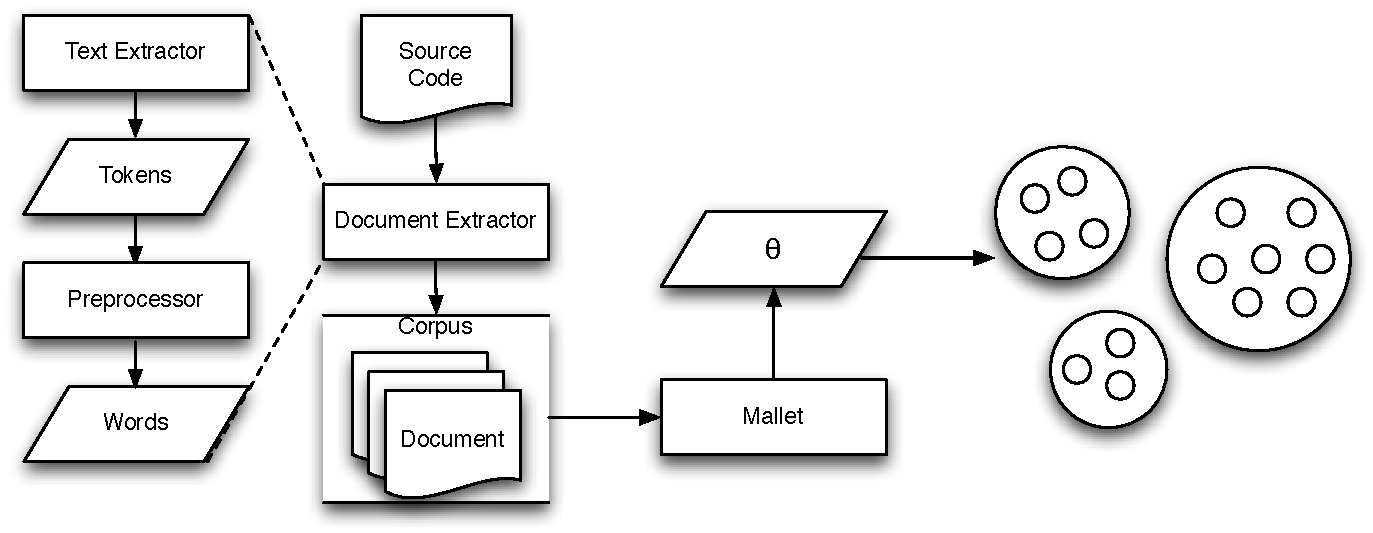
\includegraphics[width=.8625\textwidth]{Clustering}}
\caption{The source code document extraction and topic modeling processes.}
\label{fig:extract}
\vspace{-2mm}
\end{figure*}

The left side of Figure~\ref{fig:extract} illustrates the source code
document extraction process.
A document extractor takes source code as input and produces a corpus as
output.
Each document in the corpus contains the words associated with a class.
The text extractor is the first part of the document extractor.
It parses the source code and produces a token stream for each class.
With regard to Java, we consider interfaces, enumerations, and
annotations to be a class.
The preprocessor is the second part of the document extractor.
It applies a series of transformations to each token and
produces one or more words from the token.
The transformations~\cite{Marcus-etal:04,Marcus-Menzies:10}: % that we use are:
\begin{itemize}
    \item {\it Splitting}: separate tokens into constituent words
        based on common coding style conventions (e.g., the use of camel case or underscores)
        and on the presence of non-letters (e.g., punctuation or digits)
    \item {\it Normalizing}: replace each upper case letter with the corresponding
        lower case letter
    \item {\it Filtering}: remove common words such as articles (e.g., `an' or `the'),
        programming language keywords, standard library entity names, or short words
    \item {\it Stemming}: \attn{xxxxx} 
\end{itemize}
We build a corpus from a single snapshot of a software system and for all
commits leading up to that snapshot.
In particular, for the study we present in this paper,
we use the commit or tag corresponding to the snapshot (release) of each subject system.

\subsubsection{Changesets}

For changesets, the linguistic model remains mostly the same. However,
instead of parsing source code, the changeset itself is parsed.
Figure~\ref{fig:diff} shows an example of what a changeset might look
like.
In a changeset, we do not parse any further for source code entities.
A changeset, ideally, represents a single feature modification, addition, or deletion, which may crosscut many source code entities.


%diff --git a/lao b/tzu
%index 635ef2c..5af88a8 100644
%--- a/lao
%+++ b/tzu
\begin{figure}[ht]
\centering
\footnotesize
\begin{lstlisting}[language=diff, basicstyle=\ttfamily]
--- lao
+++ tzu
@@ -1,7 +1,6 @@
-The Way that can be told of is not the eternal Way;
-The name that can be named is not the eternal name.
 The Nameless is the origin of Heaven and Earth;
-The Named is the mother of all things.
+The named is the mother of all things.
+
 Therefore let there always be non-being,
   so we may see their subtlety,
 And let there always be being,
@@ -9,3 +8,6 @@ And let there always be being,
 The two are the same,
 But after they are produced,
   they have different names.
+They both may be called deep and profound.
+Deeper and more profound,
+The door of all subtleties!
\end{lstlisting}
\caption{Example of a \texttt{git diff}.
Black or blue lines denote metadata about the change useful for patching.
In particular, black lines represent context lines (beginning with
a single space).
Red lines (beginning with
a single~\texttt{-}) denote line removals, and green lines (beginning
with a single~\texttt{+}) denote line additions.}
\label{fig:diff}
\vspace{-10pt}
\end{figure}

\subsection{Topic Modeling}
\label{sec:topicmodeling}

\subsubsection{Snapshots}

\begin{enumerate}
    \item Build a topic model from a corpus
    \item Query the model
    \item Rank the source code entities by how similar their doc-topic is to the query's.
\end{enumerate}

\subsubsection{Changesets}

\begin{enumerate}
    \item Build model from changeset corpus
    \item \emph{Do not} infer a $\theta_{changesets}$
    \item Infer a $\theta_{source code}$ from the source code corpus
    \item On a new change:
        \begin{itemize}
            \item Update the model with new changeset
            \item Update $\theta_{source code}$ with the new inferrence of the changed source code entity
        \end{itemize}
\end{enumerate}


